\documentclass[letterpaper,9pt,twocolumn,twoside,]{pinp}

%% Some pieces required from the pandoc template
\providecommand{\tightlist}{%
  \setlength{\itemsep}{0pt}\setlength{\parskip}{0pt}}

% Use the lineno option to display guide line numbers if required.
% Note that the use of elements such as single-column equations
% may affect the guide line number alignment.

\usepackage[T1]{fontenc}
\usepackage[utf8]{inputenc}

% pinp change: the geometry package layout settings need to be set here, not in pinp.cls
\geometry{layoutsize={0.95588\paperwidth,0.98864\paperheight},%
  layouthoffset=0.02206\paperwidth, layoutvoffset=0.00568\paperheight}

\definecolor{pinpblue}{HTML}{185FAF}  % imagecolorpicker on blue for new R logo
\definecolor{pnasbluetext}{RGB}{101,0,0} %



\title{Linear Regression on New York Housing Data}

\author[]{}


\setcounter{secnumdepth}{0}

% Please give the surname of the lead author for the running footer
\leadauthor{}

% Keywords are not mandatory, but authors are strongly encouraged to provide them. If provided, please include two to five keywords, separated by the pipe symbol, e.g:
 

\begin{abstract}
Multiple linear regression was used to attempt to accurately, yet
robustly predict house prices with given attributes. Our model found
that the presence of a waterfront, central air-conditioning, construct
type and the number of bathrooms was associated with a large impact on
house price. Unexpectedly, new constructs have a negative influence on
price. This requires further examination. Our final model of 9
predictors out of 16 had a MAE of 41443, the best out of our tested
models. Limitations and additional variables that may improve
performance are identified.
\end{abstract}

\dates{Sourish Iyengar}


% initially we use doi so keep for backwards compatibility
% new name is doi_footer

\pinpfootercontents{DATA2902}

\begin{document}

% Optional adjustment to line up main text (after abstract) of first page with line numbers, when using both lineno and twocolumn options.
% You should only change this length when you've finalised the article contents.
\verticaladjustment{-2pt}

\maketitle
\thispagestyle{firststyle}
\ifthenelse{\boolean{shortarticle}}{\ifthenelse{\boolean{singlecolumn}}{\abscontentformatted}{\abscontent}}{}

% If your first paragraph (i.e. with the \dropcap) contains a list environment (quote, quotation, theorem, definition, enumerate, itemize...), the line after the list may have some extra indentation. If this is the case, add \parshape=0 to the end of the list environment.


\hypertarget{introduction-dataset-description}{%
\subsection{Introduction \& Dataset
Description}\label{introduction-dataset-description}}

\hfill\break
\noindent When buying, developing or investing in properties, it can be
difficult to decide what factors are important in maximising
affordability or returns. Furthermore, house appraisals can be time
consuming, expensive and prone to human error. Thus, our analysis aims
to determine a systematic relationship between variables found in a
housing dataset and their price using a multiple linear regression
model.\\
~\\
\noindent The dataset used was collected by Candice Corvetti, and is a
random sample of 1734 houses in Saratoga County, New York in 2006. It
contains 16 explanatory variables that relate to the size, age, room
types, land value and categorical features of a house. These variables
and their abbreviated names are described in A1.\\

\vspace{-5pt}

\hypertarget{initial-filtering-and-variable-transformations}{%
\subsection{Initial Filtering and Variable
Transformations}\label{initial-filtering-and-variable-transformations}}

\hfill\break
House prices by category was observed. From A2, not having heating or
fuel type is associated with lower prices relative to other categories
for their respective variables. To aid with model interpretability, they
were collapsed into binary variables that do or do not have
heating/fueling. From A3,the prices across categories in the test and
sewer type variables didn't seem to differ drastically. Thus, these
variables are not fitted in the following models. The other categorical
variables are visualised in A4.\\
~\\
\noindent Relative to the age, \(log(age+1)\) had a more pairwise linear
relationship with price and thus was transformed. From A5, lot size,
bedrooms and percentage college were dropped as they did not seem to be
linear with price even after using a log transformation.\\
~\\
\noindent All the assumptions of linear regression were satisfied on the
full model. These will be verified again after the final model is
selected.

\hypertarget{model-selection}{%
\subsection{Model Selection}\label{model-selection}}

\hypertarget{stepwise-regression}{%
\subsubsection{Stepwise Regression}\label{stepwise-regression}}

\hfill\break
Backward and forward stepwise regression was performed. This involves a
non-exhaustive construction of a regression model that iteratively drops
(backward selection ) or adds (foward selection) parameters to minimise
the AIC score. Both methods of stepwise regression dropped fuel type and
fireplace from the final model.

\hypertarget{model-stability}{%
\subsubsection{Model Stability}\label{model-stability}}

\hfill\break
The variable inclusion plot varies the value of the penalty coefficient,
\(\lambda\), on the x-axis. On the y-axis, the probability a parameter
is included in models that minimise the loss plus penalty in 150
weighted bootstrap samples is observed. This is done to see the effect
of slight deviations in our samples in the selection of various
parameters. If stable, the probability a parameter is selected should be
relatively consistent as \(\lambda\) is varied.

\vspace{-10pt}

\begin{center}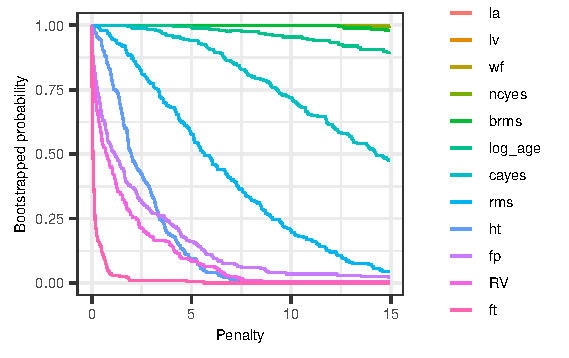
\includegraphics{Report_files/figure-latex/unnamed-chunk-8-1} \end{center}
\vspace{-10pt}

\centerline{\small Figure 1:  Variable Inclusion Plot}
\smallskip

\noindent In Figure 1, \texttt{RV} is a redundant variable independent
of price. Lines following a similar path to \texttt{RV} such as
\texttt{ft},\texttt{ht} and \texttt{fp} aren't likely to be in a stable
model. Conversely, \texttt{la}, \texttt{lv}, \texttt{wf}, \texttt{nc},
\texttt{brms}, \texttt{ca} and \texttt{log\_age} are selected with
relatively high probability throughout. The probability that the
\texttt{rms\textquotesingle{}s} variable is selected converges to 0 as
\(\lambda\) increases. However, this occurs relatively slowly. This is
investigated using model stability plots (MSPs).\\
~\\
\noindent In MSPs, \(\lambda = 2\) is fixed, a circle represents a model
and its size is proportional to its stability in the bootstrap samples.

\vspace{-15pt}

\begin{center}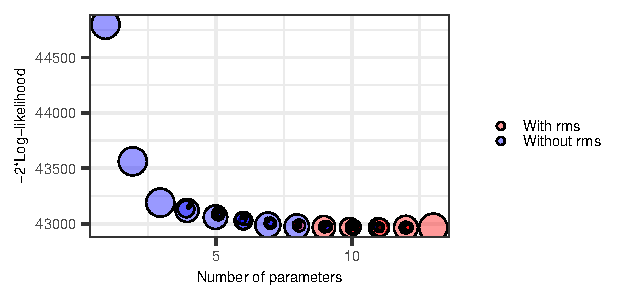
\includegraphics{Report_files/figure-latex/unnamed-chunk-10-1} \end{center}

\vspace{-10pt}

\centerline{\small Figure 2: Model Stability Plot}
\smallskip

\noindent From Figure 2, the model selected through stepwise regression
isn't overwhelmingly dominant in its dimension, \(k=10\). Contrastingly,
rooms is selected in a clear dominant model of \(k=9\). There are also
stable models of \(k=\text{5,7,8}\) with comparable probabilities of
selection. However, this is empirically stronger for the model of size 8
as it is in a higher dimension.\\
~\\
\noindent We proceed with the stable dominant models of
\(k \in \text{{8,9}}\) for model evaluation.

\hypertarget{model-evaluation---k-fold-cross-validation}{%
\subsection{Model Evaluation - K-fold Cross
Validation}\label{model-evaluation---k-fold-cross-validation}}

\begin{center}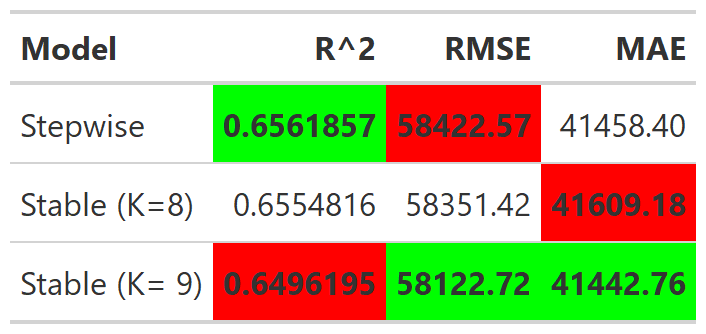
\includegraphics[width=210px,height=90px]{Rdata_Files/model_comparison_table} \end{center}
\vspace{-7pt}
\centerline{\small Figure 3: 10-fold CV-Out of Sample Performance}

\hfill\break
\noindent  Figure 3 shows that on average, the dimension 9 stable model
had the best out of sample performance in 2/3 metrics. Although it had
the lowest \(R^2\) value, relative to the stepwise and dimension 8
model, it performs better regardless of whether large errors are
penalised to a greater extent. This is indicated by its MAE and RMSE
score. Compared to \(R^2\), RMSE and MAE are easier to interpret for
non-statisticians. Thus, we chose to proceed with the dimension 9 model
as it performs the best for these metrics.

\begin{center}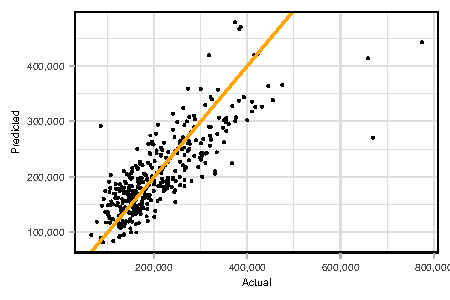
\includegraphics{Report_files/figure-latex/unnamed-chunk-14-1} \end{center}
\vspace{-10pt}
\centerline{\small Figure 4: Out of sample Actual vs Predicted Plot}

\hfill\break
\noindent Figure 4 displays the out of sample performance of the stable
dimension 9 model on 20\% of the data. The position of the three houses
on the far right indicate that they may be overpriced, relative to the
other houses. Further exploration of these observations may reveal other
factors that influence house prices.

\hypertarget{assumptions-of-the-final-selected-model}{%
\subsection{Assumptions of the Final Selected
Model}\label{assumptions-of-the-final-selected-model}}

\hfill\break
Assumptions of linear regression must be satisfied to ensure it is
appropriate to fit a linear model and inferences are valid. They are
linearity between predictors and price, homoscedasticity, independence
and normality in the error distribution.\\
~\\
\noindent From A6, there is pairwise linearity between predictors
against price. In A7, the residuals are symmetrically distributed about
0, indicating multivariate linearity is satisfied.\\
~\\
\noindent The residuals in A7 with a value above 250,000 may indicate
heteroskedasticity. These points are a small proportion of the dataset
and are unlikely to have a detrimental impact on inferences. Thus, we
proceed with this assumption being satisfied.\\

\noindent In A7, the residuals don't fall on the lower and upper tail of
the qqnorm diagonal line, indicating non-normality. However, since the
sample size is large \((n = 1734)\), we rely on the Central Limit
Theorem for approximately valid inferences.\\
~\\
\noindent Independence is assumed by the method of data collection.

\hypertarget{interpreting-coefficients}{%
\subsection{Interpreting Coefficients}\label{interpreting-coefficients}}

\hfill\break
\small
\[\operatorname{price} = 33317.24 + 67.21(\operatorname{living area}) + 19367.65(\operatorname{bathrooms})\]
\[+0.93(\operatorname{land value}) - 9226.81(\operatorname{\log(age)}) + 122570.59(\operatorname{waterfront}_{\operatorname{yes}})\]
\[-59575.95(\operatorname{new construct}_{\operatorname{yes}}) + 12562.28(\operatorname{central air}_{\operatorname{yes}})\]
\[+ 2183.2(\operatorname{rooms})\, + \epsilon\] \normalsize
\noindent The intercept and all coefficients were found to significantly
differ from 0 at a 5\% significance level. The intercept of the final
model is not interpretable in the context of the domain, as a house
cannot exist when all the other parameters are 0.\\
~\\
\noindent There are positive coefficients for living area, bathrooms,
land value, waterfront, central air conditioning and rooms. In this
model, these are the distinguishable features of higher end houses. As
expected, an increase in one dollar of land value is approximate to one
dollar of price. Comparing the magnitude of coefficients reveals that
bathrooms have a stronger weight than rooms with regards to the house
price. The majority of homes have more rooms than bathrooms and this is
reflected in the model. Additionally, waterfront, new construct,
bathrooms and central air conditioning are associated with a relatively
high magnitude of impact on price.\\
~\\
\noindent There are negative coefficients for log age and new construct.
A 1\% increase in age is correlated with a \$92 decrease in price.
Interestingly, new constructs lower the price of the house. This may be
confounded by other underlying variables such as house type or location,
as newer constructions are typically multi-dwellings or built further
from the urban centre.

\hypertarget{limitations-conclusion-and-further-study}{%
\subsection{Limitations, Conclusion and Further
Study}\label{limitations-conclusion-and-further-study}}

\hfill\break
Since the data was sourced in 2006, our analysis may not be valid in
2020. House prices also tend to fluctuate with global economic
conditions but this is not accounted for in our model. Additionally, the
data only contains samples from houses in Saratoga, so our analysis may
not apply to outside this region. It would also be inappropriate to
predict the value of houses with attributes differing from what the
model was trained on.\\
~\\
\noindent In conclusion, we developed a stable final model that that
performs fairly well in predicting house prices and may be fine-tuned
further prior to deployment. An appropriate further investigation would
be the location and type of newly constructed homes. We could scrutinise
the abnormal points from Figure 4 to gain further insight. Additionally,
having a wider range of attributes such as proximity to public
transport,schools, the neighbourhood crime rates, and more housing data
beyond Saratoga, would allow for a more robust model to be developed.

\hypertarget{references}{%
\subsection{References}\label{references}}

\hfill\break
\indent Corvetti, C. (2020). SaratogaHouses: Houses in Saratoga County
(2006). mosaicData: Project MOSAIC Data Sets.
\url{https://rdrr.io/cran/mosaicData/man/SaratogaHouses.html}

Kuhn, M. (2020). caret: Classification and Regression Training. R
package version 6.0-86. \url{https://CRAN.R-project.org/package=caret}

Tarr G, Müller S, Welsh AH (2018). ``mplot: An R Package for Graphical
Model Stability and Variable Selection Procedures.'' \emph{Journal of
Statistical Software}, \emph{83}(9), 1-28. doi: 10.18637/jss.v083.i09
(URL: \url{https://doi.org/10.18637/jss.v083.i09}).

Wickham et al., (2019). Welcome to the tidyverse. Journal of Open Source
Software, 4(43), 1686, \url{https://doi.org/10.21105/joss.01686}

\hypertarget{appendix}{%
\subsection{Appendix}\label{appendix}}

\begin{center}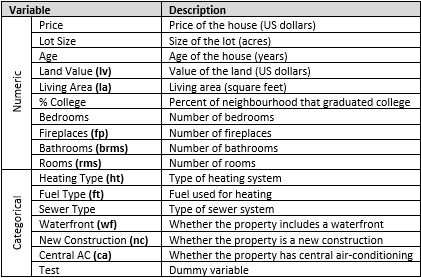
\includegraphics[width=250px]{Rdata_Files/variabletable} \end{center}
\centerline{\small A1. Dataset Variable Descriptions}

\begin{center}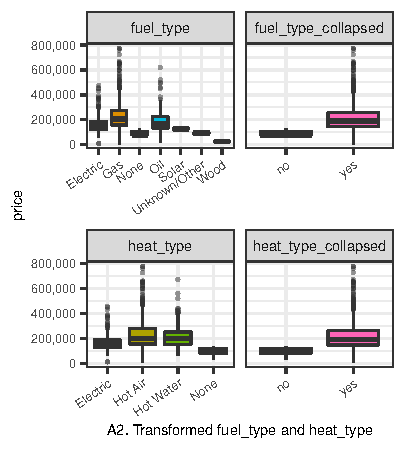
\includegraphics{Report_files/figure-latex/unnamed-chunk-20-1} \end{center}
\vspace{-20pt}

\begin{center}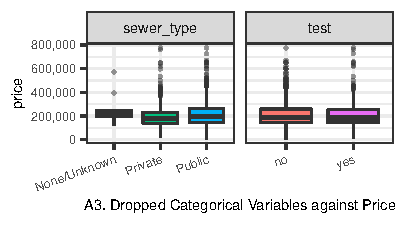
\includegraphics{Report_files/figure-latex/unnamed-chunk-21-1} \end{center}
\vspace{-20pt}

\begin{center}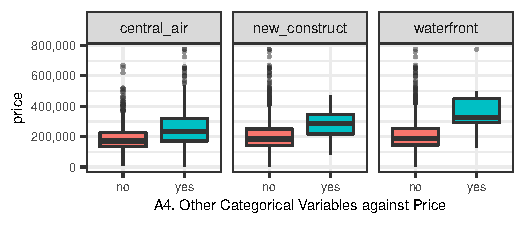
\includegraphics{Report_files/figure-latex/unnamed-chunk-22-1} \end{center}

\vspace{-20pt}

\begin{center}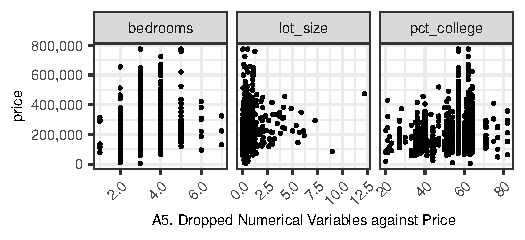
\includegraphics{Report_files/figure-latex/unnamed-chunk-23-1} \end{center}

\begin{center}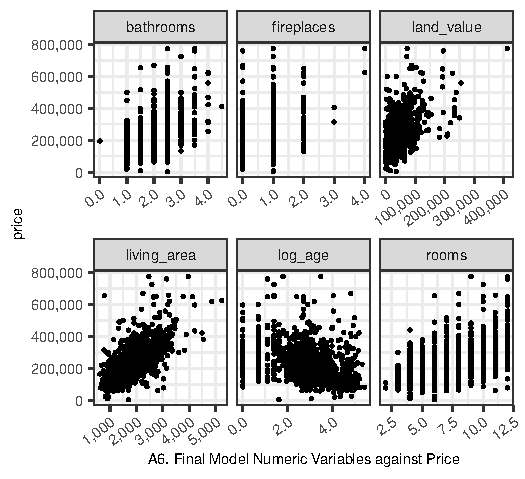
\includegraphics{Report_files/figure-latex/unnamed-chunk-24-1} \end{center}

\begin{center}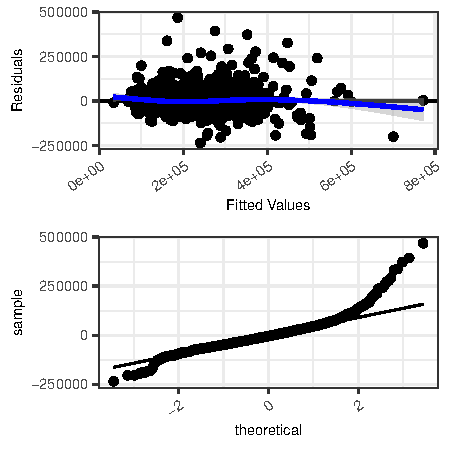
\includegraphics{Report_files/figure-latex/unnamed-chunk-25-1} \end{center}
\centerline{\small A7: Residual v.s. Fitted Plot and Normal QQplot of the Residuals}

%\showmatmethods





\end{document}
